\documentclass{assignment}
\usepackage{amsmath}
\usepackage{graphicx}
\usepackage{hyperref}
\usepackage{listings}
\usepackage{float}
\lstset{
numbers=left
}

\coursetitle{Computer Vision II}
\courselabel{CSE 252B}
\exercisesheet{Homework 1}{}
\student{Zhu, Zhongjian}
\university{University of California, San Diego}
\semester{Winter 2017}
\date{\today}

\begin{document}
\begin{problemlist}

\pbitem Line-plane intersection

The line in 3D defined by the join of the points $\mathbf{X_1} = (X_1,Y_1,Z_1,T_1)^ \mathrm{T}$ and $\mathbf{X_2} = (X_2,Y_2,Z_2,T_2)^ \mathrm{T}$ can be represented as a Pl\"ucker matrix L = $\mathbf{X_1X_2^ \mathrm{T} - X_2X_1^ \mathrm{T}}$ or pencil of points $\mathbf{X}(\lambda) = \lambda\mathbf{X_1} + (1 - \lambda)\mathbf{X_2}$. The line intersects the plane $\mathbf{\pi} = (a,b,c,d)^\mathrm{T}$ at the point $\mathbf{X_\mathrm{L}} = \mathrm{L}\pi$ or $\mathbf{X}(\lambda_\pi)$, where $\lambda_\pi$ is determined such that $\mathbf{X}(\lambda_\pi)^\mathrm{T}\pi = 0$. Show that $\mathbf{X}_\mathrm{L}$ is equal to $\mathbf{X}(\lambda_\pi)$ up to scale.
\\
\\
\textbf{Solution}\\
Since $\mathbf{X_\mathrm{L}} = \mathrm{L}\pi$, then
\[ \mathbf{X_\mathrm{L}} = (\mathbf{X_1X_2^ \mathrm{T} - X_2X_1^ \mathrm{T}})\pi =
\begin{bmatrix}
b(X_1Y_2-X_2Y_1)&+&c(X_1Z_2 - X_2Z_1)&+&d(T_2X_1 - T_1X_2)\\
a(X_2Y_1-X_1Y_2)&+&c(T_1Z_2 - Y_2Z_1)&+&d(T_2Y_1 - T_1Y_2)\\
a(X_2Z_1-X_1Z_2)&+&b(Y_2Z_1 - Y_1Z_2)&+&d(T_2Z_1 - T_1Z_2)\\
a(T_1X_2-T_2X_1)&+&b(T_1T_2 - T_2Y_1)&+&c(T_1Z_2 - T_2Z_1)\end{bmatrix}.\]
For $\mathbf{X}(\lambda_\pi)$, from $\mathbf{X}(\lambda_\pi)^\mathrm{T}\pi = 0$, we have
\[ \lambda_\pi = -\frac{aX_2+bY_2+cZ_2+dT_2}{a(X_1-X_2)+b(Y_1-Y2)+c(Z_1-Z_2)+d(T_1-T2)}.\]Let $m = a(X_1-X_2)+b(Y_1-Y2)+c(Z_1-Z_2)+d(T_1-T2)$, then
\[\mathbf{X}(\lambda_\pi) = -\frac{1}{m}
\begin{bmatrix}
b(X_1Y_2-X_2Y_1)&+&c(X_1Z_2 - X_2Z_1)&+&d(T_2X_1 - T_1X_2)\\
a(X_2Y_1-X_1Y_2)&+&c(T_1Z_2 - Y_2Z_1)&+&d(T_2Y_1 - T_1Y_2)\\
a(X_2Z_1-X_1Z_2)&+&b(Y_2Z_1 - Y_1Z_2)&+&d(T_2Z_1 - T_1Z_2)\\
a(T_1X_2-T_2X_1)&+&b(T_1T_2 - T_2Y_1)&+&c(T_1Z_2 - T_2Z_1)\end{bmatrix}.
\]
So, $\mathbf{X}_\mathrm{L} = \mathbf{X}(\lambda_\pi)$.
\\\\
\pbitem Line-quadric intersection

If the pencil of points $\mathbf{X}(\lambda) = \lambda\mathbf{X_1} + (1 - \lambda)\mathbf{X_2}$ represents a line in 3D, the (up to two) real roots of the quadratic polynomial $c_2\lambda_Q^2+c_1\lambda_Q+c_0=0$ are used to solve for the intersection point(s) $\mathbf{X}(\lambda_Q)$. Show that $c_2=\mathbf{X_1}^\mathrm{T}Q\mathbf{X_1}-2\mathbf{X_1}^\mathrm{T}Q\mathbf{X_2}+\mathbf{X_2}^\mathrm{T}Q\mathbf{X_2}$, $c_1=2(\mathbf{X_1}^\mathrm{T}Q\mathbf{X_2}-\mathbf{X_2}^\mathrm{T}Q\mathbf{X_2})$, and $c_0=\mathbf{X_2}^\mathrm{T}Q\mathbf{X_2}$.
\\\\
\textbf{Solution}\\
A 3D point $\mathbf{X}$ is on the quadric $Q$ if and only if $\mathbf{X}^\mathrm{T}Q\mathbf{X}=0$, then
\begin{equation}
(\lambda\mathbf{X_1} + (1 - \lambda)\mathbf{X_2})^\mathrm{T}Q(\lambda\mathbf{X_1} + (1 - \lambda)\mathbf{X_2})=0
\end{equation}
\begin{equation}
\lambda^2\mathbf{X_1}^\mathrm{T}Q\mathbf{X_1}+
\lambda(1-\lambda)\mathbf{X_1}^\mathrm{T}Q\mathbf{X_2}+
\lambda(1-\lambda)\mathbf{X_2}^\mathrm{T}Q\mathbf{X_1}+
(1-\lambda)^2\mathbf{X_2}^\mathrm{T}Q\mathbf{X_2}=0
\end{equation}

Since the transpose of a scalar is itself, from equation(0-1), we have
\begin{equation}
(\mathbf{X_1}^\mathrm{T}Q\mathbf{X_1}-2\mathbf{X_1}^\mathrm{T}Q\mathbf{X_2}+\mathbf{X_2}^\mathrm{T}Q\mathbf{X_2})\lambda^2+
2(\mathbf{X_1}^\mathrm{T}Q\mathbf{X_2}-\mathbf{X_2}^\mathrm{T}Q\mathbf{X_2})\lambda+
\mathbf{X_2}^\mathrm{T}Q\mathbf{X_2}=0
\end{equation}
So, $c_2=\mathbf{X_1}^\mathrm{T}Q\mathbf{X_1}-2\mathbf{X_1}^\mathrm{T}Q\mathbf{X_2}+\mathbf{X_2}^\mathrm{T}Q\mathbf{X_2}$, $c_1=2(\mathbf{X_1}^\mathrm{T}Q\mathbf{X_2}-\mathbf{X_2}^\mathrm{T}Q\mathbf{X_2})$, and $c_0=\mathbf{X_2}^\mathrm{T}Q\mathbf{X_2}$.
\\\\
\pbitem Programming: Automatic feature detection and matching

\begin{figure}[H]
  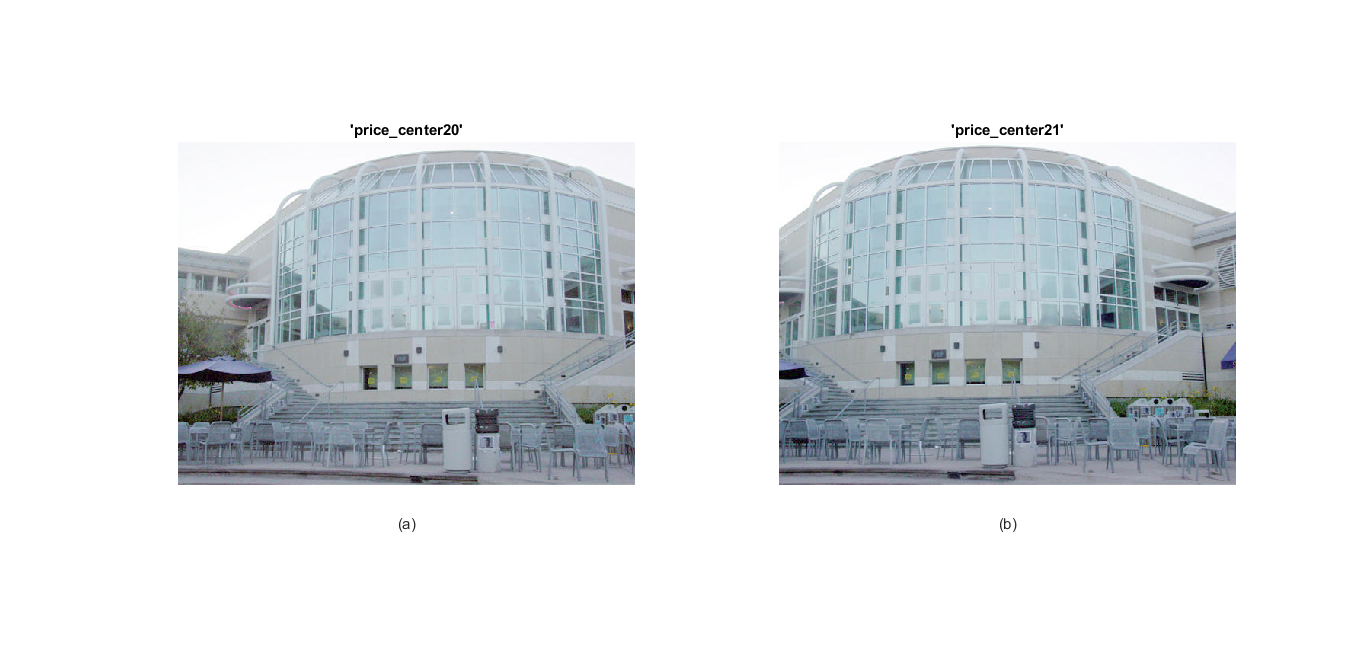
\includegraphics[width=\textwidth]{InputImage}
\caption{(a) shows the image \emph{price\_ center20.JPG}, (b) shows the image \emph{price\_ center21.JPG}.}
\label{fig:images}
\end{figure}

\begin{enumerate}
\item Feature detection\\
The size of the feature detection window is $11\times11$, 
the minor eigenvalue threshold value is 5, 
the size of the local non-maximum suppression window is $9\times9$.\\
The number of features detected in \emph{price\_ center20.JPG} is 616, and the number of features detected in \emph{price\_ center21.JPG} is 632.

\begin{figure}[H]
  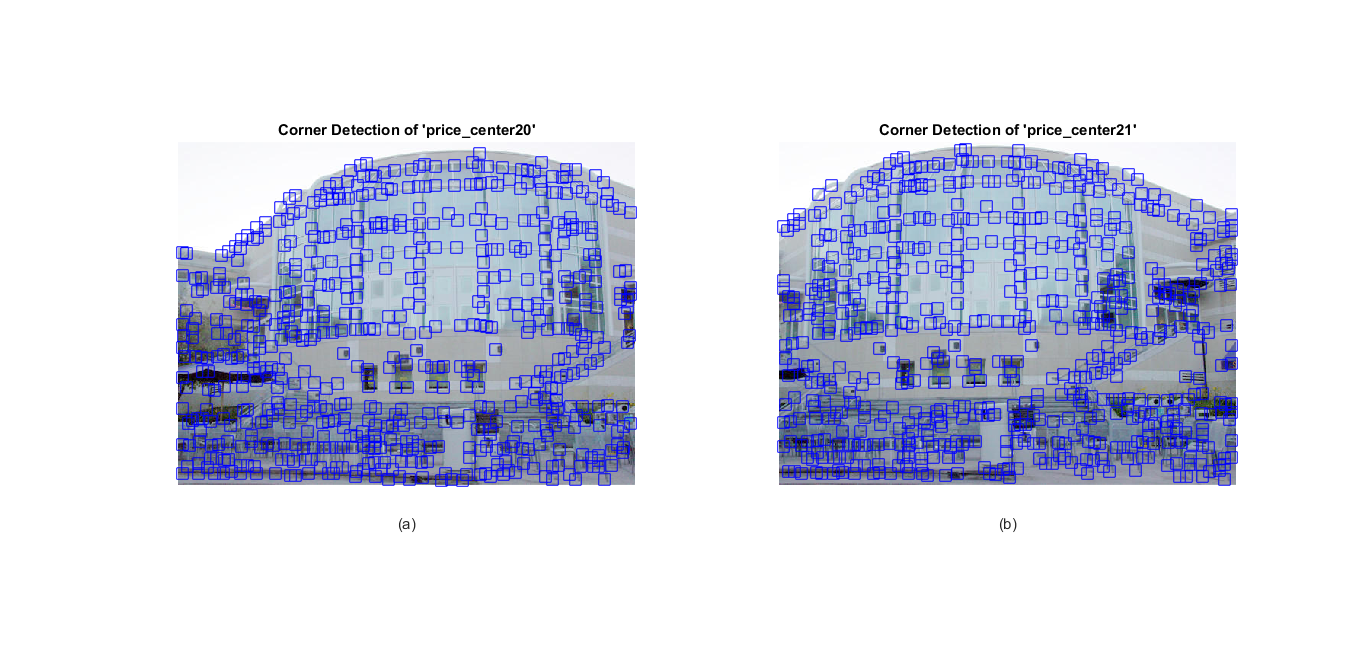
\includegraphics[width=6in]{CornerDetection_NMS}
\caption{(a) shows detected corners(after local nonmaximum suppression) of the image \emph{price\_ center20.JPG}, (b) shows detected corners(after local nonmaximum suppression) of the image \emph{price\_ center21.JPG}.}
\label{fig:images}
\end{figure}
 
\begin{figure}[H]
  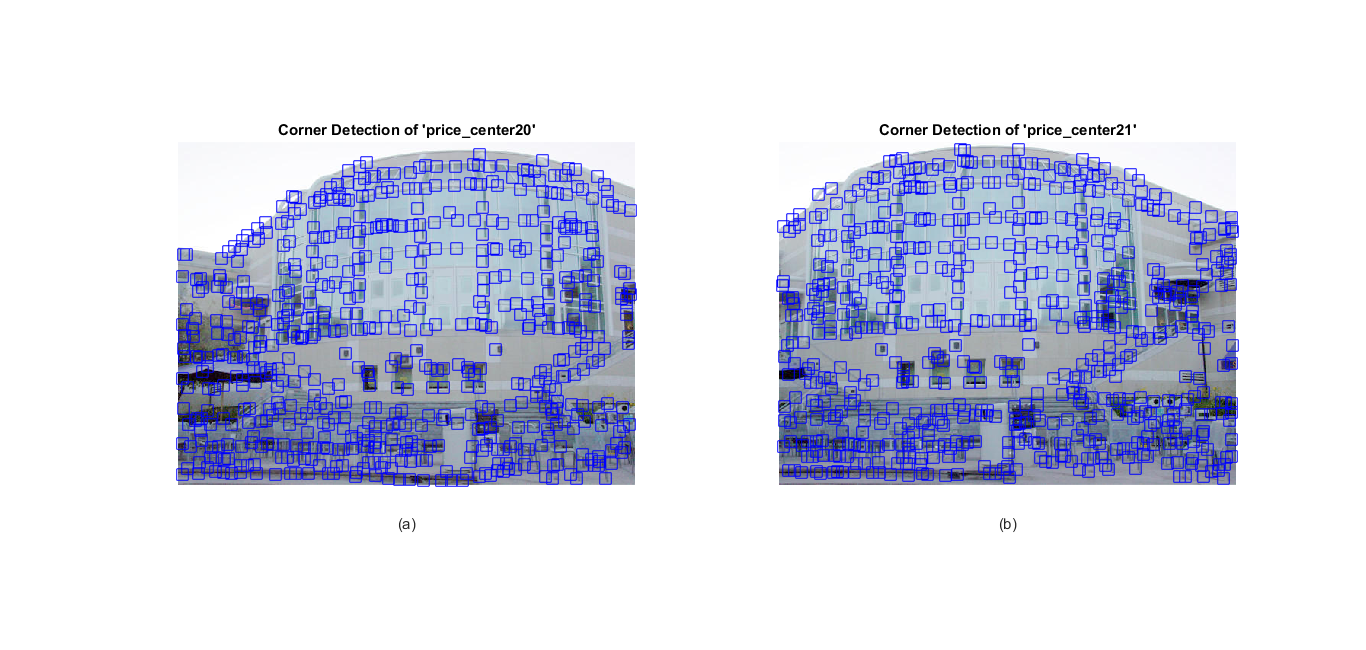
\includegraphics[width=6in]{CornerDetection_Subp}
\caption{(a) shows detected corners(about the subpixel) of the image \emph{price\_ center20.JPG}, (b) shows detected corners(about the subpixel) of the image \emph{price\_ center21.JPG}.}
\label{fig:images}
\end{figure} 




\item Feature matching\\
The size of the proximity window is $20\times500$, the correlation coefficient threshold value is 0.6, the distance ratio threshold value is 0.9, and the resulting
number of putative feature correspondences is 196.\\
\\
\begin{figure}[H]
  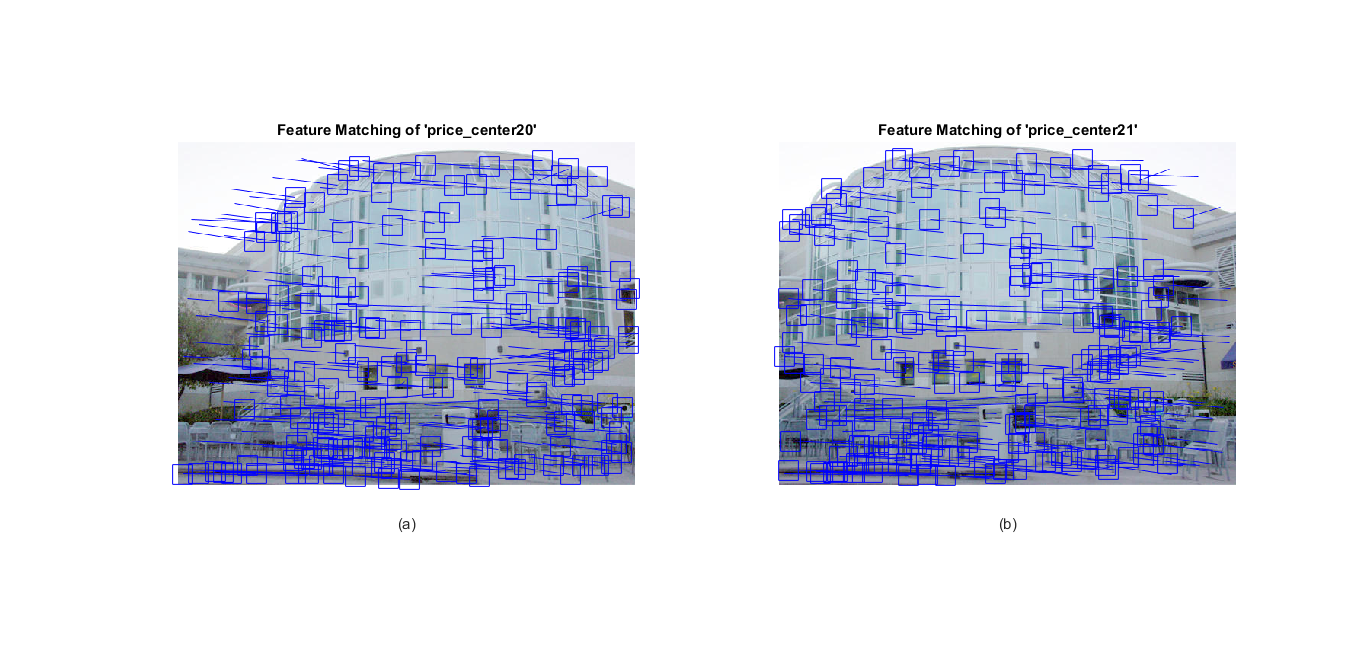
\includegraphics[width=6in]{FeatureMatch}
\caption{(a) shows matched features in \emph{price\_ center20.JPG}, (b) shows matched features in \emph{price\_ center21.JPG}.}
\label{fig:images}
\end{figure} 

\end{enumerate}
\end{problemlist}

\begin{flushleft}
\large{\textbf{Appendix}}
\end{flushleft}

\begin{lstlisting}[language=MATLAB]
close all;
clear;
clc;
%% Corner Detection
win_detect = 11;
win_spr = 9;
eigen_th = 5;
I0 = imread('price_center20.JPG');
I1 = imread('price_center21.JPG');
[r0,c0,x_f0,y_f0] = CornerCoordinate(I0,win_detect,win_spr,eigen_th);
[r1,c1,x_f1,y_f1] = CornerCoordinate(I1,win_detect,win_spr,eigen_th);

figure(1)
subplot(1,2,1)
imshow(I0);
xlabel('(a)');
title('''price\_center20''');
subplot(1,2,2)
imshow(I1);
xlabel('(b)');
title('''price\_center21''');

figure(2)
subplot(1,2,1)
imshow(I0);hold on
plot(c0,r0,'bs','MarkerSize',win_detect);hold off
xlabel('(a)');
title('Corner Detection of ''price\_center20''');
subplot(1,2,2)
imshow(I1);hold on
xlabel('(b)')
plot(c1,r1,'bs','MarkerSize',win_detect);hold off
title('Corner Detection of ''price\_center21''');

figure(3)
subplot(1,2,1)
imshow(I0);hold on
plot(y_f0,x_f0,'bs','MarkerSize',win_detect);hold off
xlabel('(a)');
title('Corner Detection of ''price\_center20''');
subplot(1,2,2)
imshow(I1);hold on
xlabel('(b)')
plot(y_f1,x_f1,'bs','MarkerSize',win_detect);hold off
title('Corner Detection of ''price\_center21''');

%% Feature Matching
win_match = 19;
simi_th = 0.6;
dist_th = 0.9;
[X0,Y0,X1,Y1] = FeatureMatch(I0,I1,x_f0,y_f0,x_f1,y_f1,win_match,simi_th,dist_th);
figure(4)
subplot(1,2,1)
imshow(insertShape(I0,'Line',[Y0 X0 Y1 X1],'Color','blue'));
hold on
plot(Y0,X0,'bs','MarkerSize',win_match);
hold off
xlabel('(a)');
title('Feature Matching of ''price\_center20''');
subplot(1,2,2)
imshow(insertShape(I1,'Line',[Y1 X1 Y0 X0],'Color','blue'));
hold on
plot(Y1,X1,'bs','MarkerSize',win_match);
hold off
xlabel('(b)');
title('Feature Matching of ''price\_center21''');
\end{lstlisting}

\begin{lstlisting}[language=MATLAB]
function [r,c,x_f1,x_f2] = CornerCoordinate(im,win1,win2,threshold)
im = double(rgb2gray(im));
A = zeros(size(im));
k = [-1 8 0 -8 1]' / 12;
imx = imfilter(im,k','symmetric');
imy = imfilter(im,k,'symmetric');
%% Gradient matrix
for i = (win1+1)/2 : size(im,1) - (win1-1)/2
    for j = (win1+1)/2 : size(im,2) - (win1-1)/2
        im_win_x = imx(i - (win1-1)/2:i + (win1-1)/2,...
                       j - (win1-1)/2:j + (win1-1)/2);
        im_win_y = imy(i - (win1-1)/2:i + (win1-1)/2,...
                       j + (win1-1)/2:j + (win1-1)/2);

        N = zeros(2,2);
        N(1,1) = sum(sum(im_win_x.^2));
        N(1,2) = sum(sum(im_win_x .* im_win_y));
        N(2,1) = N(1,2);
        N(2,2) = sum(sum(im_win_y.^2));
        N = N/win1^2;
        lambda = (trace(N) - sqrt(trace(N)^2 - 4*det(N)))/2;
        if lambda > threshold
            A(i,j) = lambda;
        end
    end
end
%% Non-maximum suppression 
B = ordfilt2(A,win1^2,ones(win1,win1));
C = (B == A & B ~= 0);
[r,c] = find(C);
x_f1 = zeros(size(r));
x_f2 = zeros(size(r));
%% find corner
for k = 1:numel(r)
    T = zeros(2,2);
    y = zeros(2,1);
    im_win_x = imx(r(k) - (win2-1)/2:r(k) + (win2-1)/2,...
                   c(k) - (win2-1)/2:c(k) + (win2-1)/2);
    im_win_y = imy(r(k) - (win2-1)/2:r(k) + (win2-1)/2,...
                   c(k) - (win2-1)/2:c(k) + (win2-1)/2);
    xx = [r(k) - (win2-1)/2 : r(k) + (win2-1)/2]' .* ones(win2);
    yy = [c(k) - (win2-1)/2 : c(k) + (win2-1)/2] .* ones(win2);
    
    y(1) = sum(sum( xx.*im_win_x.^2 + yy.*im_win_x.*im_win_y ));
    y(2) = sum(sum( xx.*im_win_x.*im_win_y + yy.*im_win_y.^2 ));
    T(1,1) = sum(sum(im_win_x.^2));
    T(1,2) = sum(sum(im_win_x .* im_win_y));
    T(2,1) = T(1,2);
    T(2,2) = sum(sum(im_win_y.^2));
    x = T\y;
    
    x_f1(k) = x(1);
    x_f2(k) = x(2);
end
end
\end{lstlisting}
\begin{lstlisting}[language=MATLAB]
function [X0,Y0,X1,Y1] = FeatureMatch(im0,im1,x0,y0,x1,y1,win,simi_th,dist_th)
im0 = double(rgb2gray(im0));
im1 = double(rgb2gray(im1));
half_win = (win-1)/2;
%%
xx0 = x0+half_win;
xx1 = x1+half_win;
yy0 = y0+half_win;
yy1 = y1+half_win;
im0 = padarray(im0,[half_win,half_win],'symmetric');
im1 = padarray(im1,[half_win,half_win],'symmetric');
%% Xcorrelation matrix
xc = zeros(numel(xx0),numel(xx1));
crd = zeros(numel(xx0),numel(xx1));
for i = 1:numel(xx0)
    X = fix(xx0(i)) - half_win:ceil(xx0(i)) + half_win;
    Y = fix(yy0(i)) - half_win:ceil(yy0(i)) + half_win;
    im0_win = im0(X,Y);
    [X,Y] = meshgrid(X,Y);
    [Xq,Yq] = meshgrid(xx0(i)-half_win:xx0(i)+half_win,...
                       yy0(i) - half_win:yy0(i) + half_win);
    im0_win_intep = interp2(X,Y,im0_win,Xq,Yq,'linear');    

    for j = 1:numel(xx1)
        X = fix(xx1(j)) - half_win:ceil(xx1(j)) + half_win;
        Y = fix(yy1(j)) - half_win:ceil(yy1(j)) + half_win;
        im1_win = im1(X,Y);
        [X,Y] = meshgrid(X,Y);
        [Xq,Yq] = meshgrid(xx1(j)-half_win:xx1(j)+half_win,...
                           yy1(j) - half_win:yy1(j) + half_win);
        im1_win_intep = interp2(X,Y,im1_win,Xq,Yq,'linear');
        xc(i,j) = corr2(im0_win_intep,im1_win_intep);
    end
end
%% One-to-One Matching
while max(xc(:)) > simi_th
    [r,c] = find(xc == max(xc(:)));
    i = r(1);
    j = c(1);
    mx = xc(i,j);
    xc(i,j) = -1;
    next_mx = max(max(xc(i,:),[],2),max(xc(:,j)));
    
    if (1-mx) < (1-next_mx)*dist_th
        crd(i,j) = 1;
    end
    xc(i,:) = -1;
    xc(:,j) = -1;
end
[i,j] = find(crd);
X0 = x0(i);
Y0 = y0(i);
X1 = x1(j);
Y1 = y1(j);

w = abs(X0-X1);
d = abs(Y0-Y1);
n = find(w>20 | d >500);
X0(n) = [];
Y0(n) = [];
X1(n) = [];
Y1(n) = [];
end
\end{lstlisting}
\end{document}
